\chapter{Le problème : Wave Function Collapse}
\label{chap:probleme_wfc}

\section{Origine et intuition}

\subsection{De la mécanique quantique à la génération procédurale}

Le \textbf{Wave Function Collapse} (WFC) tire son nom d'une analogie avec la mécanique quantique. Dans une expérience de pensée comme le chat de Schrödinger, le système reste en \textit{superposition} de plusieurs états (vivant et mort) jusqu'à ce qu'une mesure le fasse \textit{collapser} dans un état unique. WFC applique cette image à la génération procédurale : chaque cellule de la grille de sortie commence en superposition de toutes les valeurs possibles, puis se collapse progressivement par propagation de contraintes locales \cite{heaton2018wfc}.

L'algorithme a été publié par Maxim Gumin en 2016 \cite{gumin2016wfc} sous licence MIT et a connu un succès important : il est utilisé dans des jeux commerciaux comme \textit{Townscaper}, \textit{Caves of Qud}, \textit{Bad North}, et dans de nombreux outils de level design.

\subsection{Le problème en termes formels}

Soit $S$ une grille rectangulaire de taille $r_S \times c_S$ à valeurs dans un alphabet $\Sigma$ (typiquement $\{0, 1\}$ pour le cas binaire, ou $\{0, 1, \ldots, K-1\}$ pour le cas multi-valeurs). Soit $N \in \mathbb{N}^*$ la taille de tuile, et $G$ une grille de taille $r_G \times c_G$ à valeurs dans $\Sigma$ que l'on cherche à construire.

\begin{definition}[Sous-bloc $N \times N$]
Un \textbf{sous-bloc} de taille $N \times N$ d'une grille $H$ à la position $(r, c)$ est l'ensemble des valeurs $H[(r+i) \bmod r_H][(c+j) \bmod c_H]$ pour $0 \leq i, j < N$, avec wrap-around toroïdal.
\end{definition}

\begin{definition}[Tuile valide]
Une tuile $T$ est \textbf{valide} pour $S$ si elle apparaît au moins une fois comme sous-bloc $N \times N$ de $S$.
\end{definition}

\begin{definition}[Solution WFC]
Une grille $G$ est une \textbf{solution WFC} pour $(S, N)$ si tout sous-bloc $N \times N$ de $G$ est une tuile valide pour $S$.
\end{definition}

\subsection{Exemple littéral du sujet}

Le \texttt{README.pdf} du sujet propose l'échantillon binaire suivant ($r_S = c_S = 5$) :

\begin{verbatim}
1 0 1 1 1
1 0 1 1 1
0 0 1 1 1
0 1 1 1 1
0 0 0 0 0
\end{verbatim}

Pour $N = 2$, l'extraction non-toroïdale identifie 8 tuiles distinctes ; l'extraction \textbf{toroïdale} (notre choix de design, voir Chapitre~\ref{chap:approche}) en identifie 11. Le solveur produit ensuite une grille $G$ de taille libre (par exemple $64 \times 64$) qui ne contient localement que ces tuiles.

\begin{figure}[H]
\centering
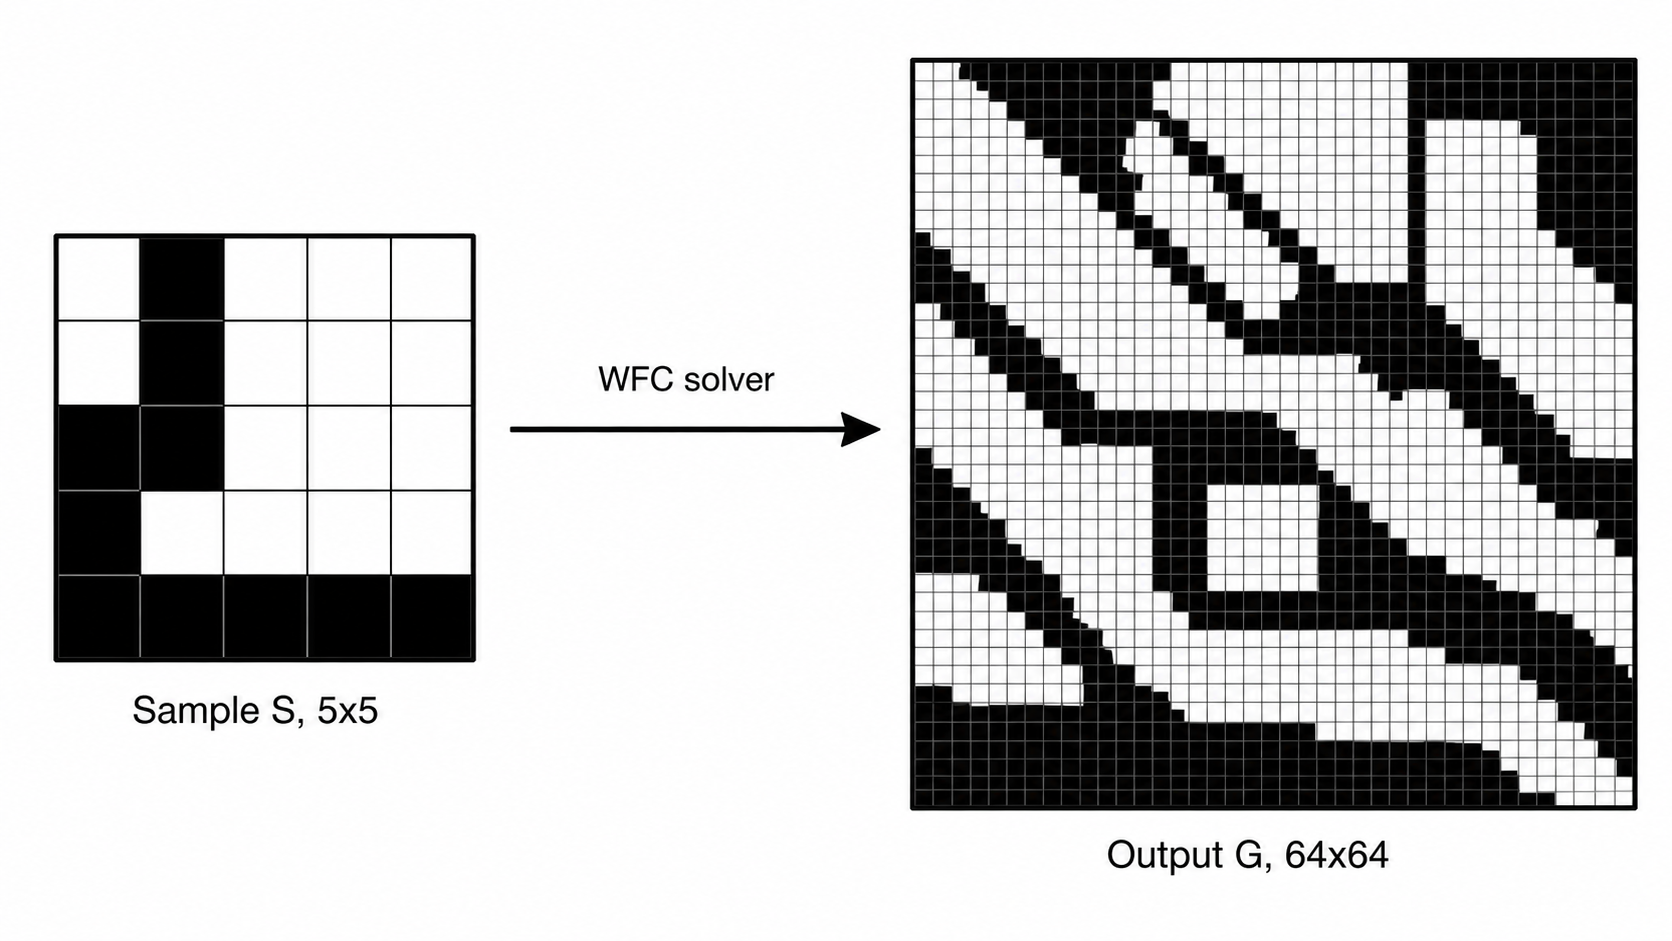
\includegraphics[width=0.85\linewidth]{results/figures/schemas/sample_to_output.png}
\caption{Pipeline WFC en une figure : à partir d'un petit échantillon $S$ (5×5), le solveur reproduit les motifs locaux dans une grille $G$ de taille libre (64×64).}
\label{fig:sample_to_output}
\end{figure}

\section{Le modèle overlapping}

WFC se décline en plusieurs variantes. Le \textbf{Simple Tiled Model} utilise une palette finie de tuiles avec contraintes d'adjacence données explicitement (utile pour les sprites de jeux). Le \textbf{Simple Tiled Model symétrique} ajoute la gestion des rotations / réflexions des tuiles. Le \textbf{modèle overlapping} (notre choix, imposé par le sujet) extrait les contraintes par recouvrement entre sous-blocs $N \times N$ de l'échantillon.

\subsection{Définition formelle des contraintes overlapping}

\begin{definition}[Compatibilité overlapping]
Deux tuiles $t_1$ et $t_2$ de taille $N \times N$ sont \textbf{compatibles} à un offset $(dx, dy)$ avec $|dx|, |dy| \leq N - 1$ si leurs valeurs coïncident sur la zone de recouvrement :
\[
\forall (x, y) \in [\max(0, -dx), \min(N-1, N-1-dx)] \times [\max(0, -dy), \min(N-1, N-1-dy)] :
\]
\[
t_1[y + dy][x + dx] = t_2[y][x]
\]
\end{definition}

Pour deux tuiles $2 \times 2$, il y a $(2N - 1)^2 = 9$ offsets pertinents (incluant $(0, 0)$ qui correspond à l'identité $t_1 = t_2$).

\subsection{Symétrie des règles}

\begin{theorem}[Symétrie des règles d'adjacence]
Pour toute paire de tuiles $(t_1, t_2)$ et tout offset $(dx, dy)$ :
\[
t_2 \in \text{allowed}(t_1, dx, dy) \iff t_1 \in \text{allowed}(t_2, -dx, -dy)
\]
\end{theorem}

Cette propriété est utilisée par notre suite de tests (\texttt{test\_overlap}) comme \textit{invariant} de validation, vérifiant en particulier que la convention d'offset est implémentée correctement (un bug subtil que nous avons détecté pendant le développement par cette voie).

% =============================================================================
\section{Applications}
\label{sec:wfc:applications}
% =============================================================================

\subsection{Jeux vidéo et level design}

WFC est massivement utilisé pour la génération procédurale de niveaux :
\begin{itemize}
    \item \textbf{Townscaper} (Oskar Stålberg, 2020) : les bâtiments sont composés en temps réel par WFC à partir d'un set de tuiles 3D.
    \item \textbf{Caves of Qud} : génération de cavernes et donjons.
    \item \textbf{Bad North} : génération des îles tactiques.
\end{itemize}

Notre démonstration UE5 (\texttt{wfc\_dungeon}, voir Chapitre~\ref{chap:extensions}) reproduit ce paradigme : génération d'un dungeon mono-étage exporté en JSON, consommé par un plugin Unreal qui spawne les meshes 3D et des actors gameplay (PlayerStart, NPC spawners, pickups) dans un \texttt{ADungeonGenerator}.

\subsection{Synthèse de textures}

WFC peut être appliqué à la synthèse de textures de grande taille à partir d'un échantillon de référence \cite{efros1999texture}. Le résultat est moins fidèle que les méthodes basées sur les réseaux de neurones (StyleGAN, etc.) mais il est entièrement déterministe et explicable.

\subsection{Inpainting et complétion}

Une extension de WFC permet le \textit{inpainting} : étant donnée une grille partiellement remplie, compléter les cellules manquantes en respectant les contraintes locales. Cette extension n'est pas implémentée dans notre projet, mais l'architecture s'y prête (il suffirait de pré-collapser certaines cellules avant de lancer le solveur).

\subsection{Création artistique}

L'algorithme est utilisé en art génératif (motifs cellulaires, mosaïques, calligraphie procédurale). Sa simplicité conceptuelle le rend accessible aux artistes non-programmeurs via des outils comme \textit{WFC Studio} ou des plugins Blender.

% =============================================================================
\section{Difficultés calculatoires}
\label{sec:wfc:difficultes}
% =============================================================================

\subsection{Espace de recherche exponentiel}

Pour une grille $r \times c$ avec $L$ tuiles candidates par cellule, l'espace de recherche brut est $L^{r \cdot c}$. Pour $L = 11$, $r = c = 128$, cela représente $11^{16384} \approx 10^{17040}$ configurations possibles. L'énumération exhaustive est exclue.

\subsection{Heuristique gloutonne}

L'algorithme de Gumin contourne cette explosion par une heuristique gloutonne en deux phases :
\begin{enumerate}
    \item \textbf{Sélection min-entropie} : choisir la cellule la plus contrainte (peu de candidats restants) avant les autres.
    \item \textbf{Propagation BFS} : après chaque collapse, propager les contraintes en intersectant les ensembles de candidats des voisins.
\end{enumerate}

L'heuristique réduit drastiquement l'espace exploré mais ne garantit pas la convergence : une succession de mauvais choix peut conduire à un \textbf{contradiction} (cellule à 0 candidats), nécessitant un retry.

\subsection{Contradictions et stratégies de récupération}

Trois stratégies sont possibles face à une contradiction :
\begin{enumerate}
    \item \textbf{Restart} (notre défaut) : abandonner la tentative, recommencer avec un nouveau seed dérivé. Simple, peu invasif, suffisant en pratique sur les samples bien comportés.
    \item \textbf{Backtracking} (notre option \texttt{--backtrack}) : revenir au dernier point de décision, essayer un autre choix. Plus puissant sur samples très contraints, plus complexe (snapshot/restore).
    \item \textbf{Soft constraints} : tolérer certaines violations à coût pondéré (non implémenté).
\end{enumerate}

\subsection{Complexité de la sélection min-entropie}

Le profilage de notre solveur série (Chapitre~\ref{chap:resultats}) révèle un résultat contre-intuitif : la \textbf{sélection min-entropie domine le temps total ($\sim 85\%$)}, pas la propagation ($\sim 12\%$). À chaque collapse, l'algorithme re-scanne toutes les $r \cdot c$ cellules pour trouver celle d'entropie minimale. Ce coût en $O(r \cdot c \cdot L)$ par collapse, multiplié par les $\sim r \cdot c$ collapses au total, donne $O((r \cdot c)^2 \cdot L)$ opérations dans la version naïve.

C'est cette étape qui justifie l'effort principal de parallélisation (\texttt{parallel\_min\_entropy} via tasks OMP).
